% See http://tex.stackexchange.com/questions/168169/options-for-supplementary-materials-in-preprint-version-revtex-arxiv

\pagebreak
\begin{center}
\textbf{\large Supplemental Materials}
\end{center}

\setcounter{equation}{0}
\setcounter{figure}{0}
\setcounter{table}{0}
% \setcounter{page}{1}
\makeatletter
\renewcommand{\theequation}{S\arabic{equation}}
\renewcommand{\thefigure}{S\arabic{figure}}
% \renewcommand{\bibnumfmt}[1]{[S#1]}
% \renewcommand{\citenumfont}[1]{S#1}

\begin{figure}
\centering
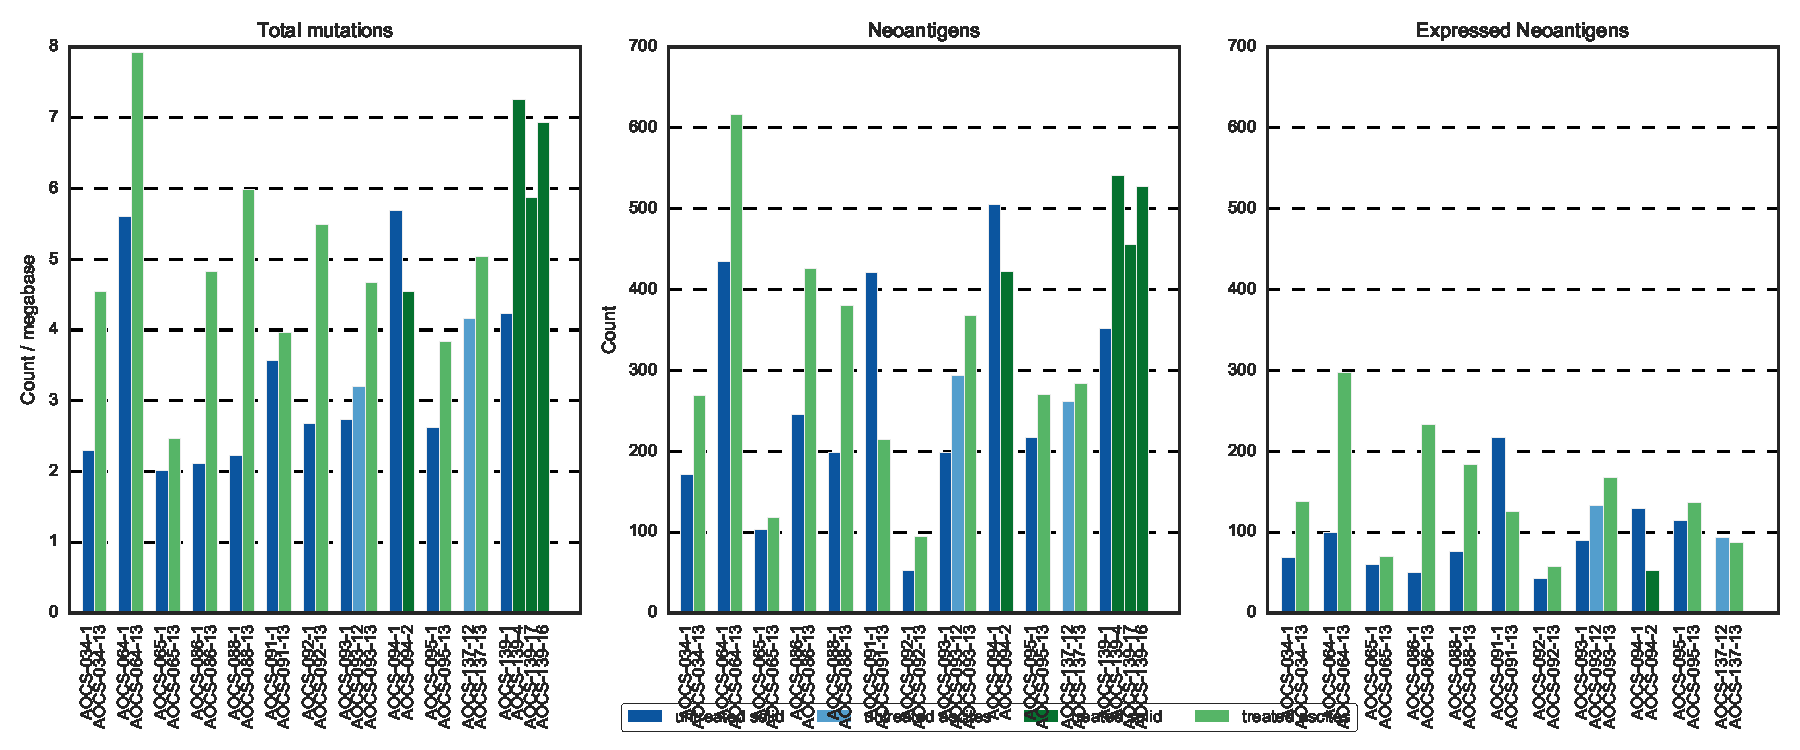
\includegraphics[scale=1.0]{figures/paired_counts.pdf}
\caption{Mutations, neoantigens, and expressed neoantigens for the donors with paired pre-/post-chemotherapy samples.}
\label{fig:supp_paired}
\end{figure}

% \usetikzlibrary{fit,positioning}
\begin{figure}
\centering
\begin{tikzpicture}
\tikzstyle{main}=[rectangle, rounded corners, minimum size = 10mm, thick, draw =black!80, node distance = 10mm]
\tikzstyle{connect}=[-latex, thick]
\tikzstyle{box}=[rectangle, draw=black!100]
  \node[main] (coefficients) [label=above:Coefficients] { $\beta \sim \mathit{N}(0, 20)$ };
  \node[main] (globalmean) [right=of coefficients,label=above:Global Mean] { $\mu_\text{global} \sim \mathit{N}(0, 100) $ };
  \node[main] (donorsigma) [right=of globalmean,label=above:Donor Variance] { $\sigma_\text{donor} \sim \mathit{Cauchy}(0, 2) $ };
  \node[main] (samplesigma) [right=of donorsigma,label=above:Sample Variance] { $\sigma_\text{sample} \sim \mathit{Cauchy}(0, 2) $ };

  \node[main] (donormean) [below=of globalmean, xshift=25mm] {$\mu_d \sim \mathit{N}(\mu_\text{global}, \sigma_\text{donor}) $};

  \node[main] (mu) [below=of donormean,label=below:] { $\mu_i = \mu_d + \beta \cdot x_i $ };
  \node[circle, thick, draw=black!80] (data) [left=10mm of mu,label=above:Observed] { $x_i$ };

  \node[main] (y) [below=of mu] {$\log y_i \sim \mathit{N}(\mu_i, \sigma_{sample})$};
  \node[circle, thick, draw=black!80] (obsy) [left=5mm of y,label=above:Observed] { $y_i$ };

  \path (globalmean) edge [connect] (donormean)
        (donorsigma) edge [connect] (donormean)
        (coefficients) edge [connect] (mu)
        (data) edge [connect] (mu)
        (obsy) edge [connect] (y)
        (donormean) edge [connect] (mu)
        (mu) edge [connect] (y)
        (samplesigma) edge [connect] (y);

  \node[rectangle, inner sep=8mm,fill=gray!100, draw=black!100, fill opacity=0.2, fit= (donormean) (y) (data) ,yshift=-3mm,xshift=1mm,label=below:$d \in \text{donors}$] {};
  \node[rectangle, inner sep=6mm,fill=gray!100, draw=black!100, fill opacity=0.2, fit= (mu) (y) (data),yshift=1mm,xshift=1mm,label=below:$i \in \text{samples($d$)}$] {};


\end{tikzpicture}
\caption{Bayesian model architecture for paired samples. For unpaired samples, $\mu_d$ is set to $\mu_\text{global}$.}
\label{fig:model_architecture}
\end{figure}

\begin{figure}[htbp]
\centering
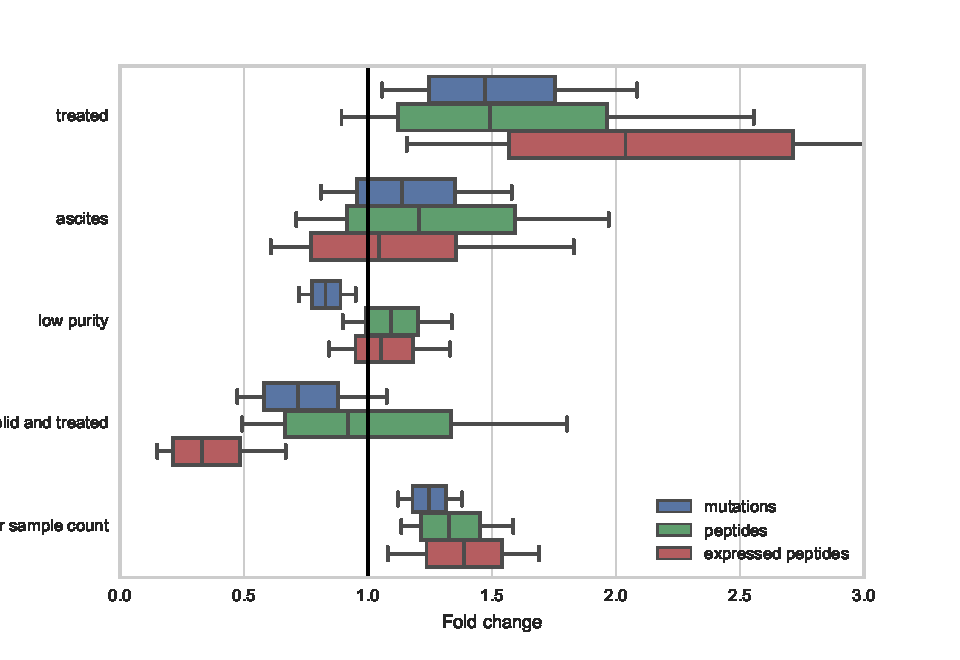
\includegraphics[scale=1.0]{figures/bayesian_model_effects.pdf}
\caption{Bayesian model effects. }
\label{fig:bayesian_model_effects}
\end{figure}

\begin{figure}[htbp]
\centering
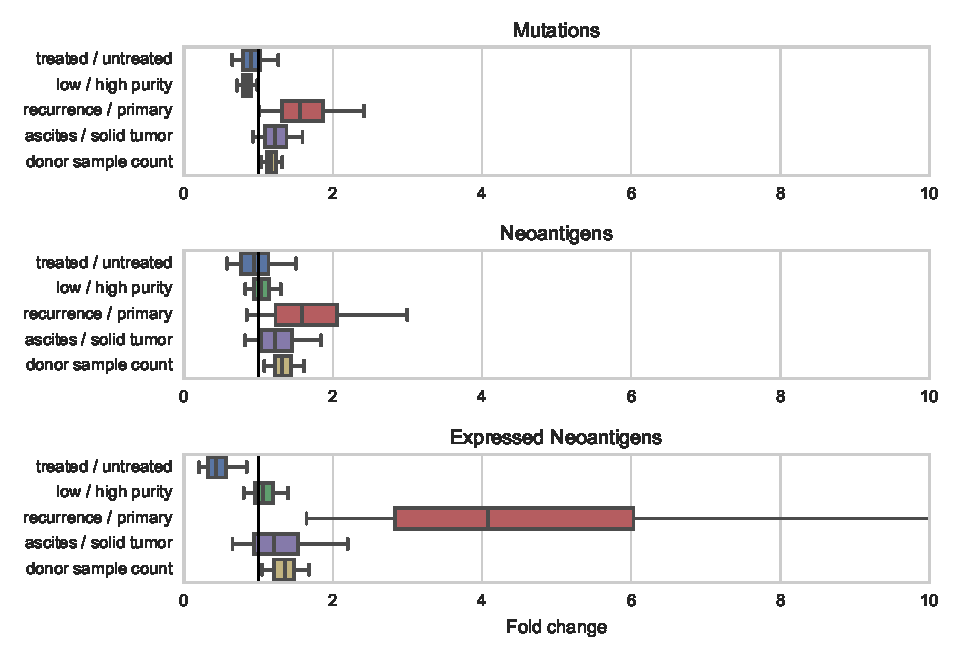
\includegraphics[scale=1.0]{figures/bayesian_model_effects_separate.pdf}
\caption{Parameter estimates for a model separating treatment effect from recurrence/relapse time-point. }
\label{fig:bayesian_model_effects_separate}
\end{figure}


\begin{figure}
\centering
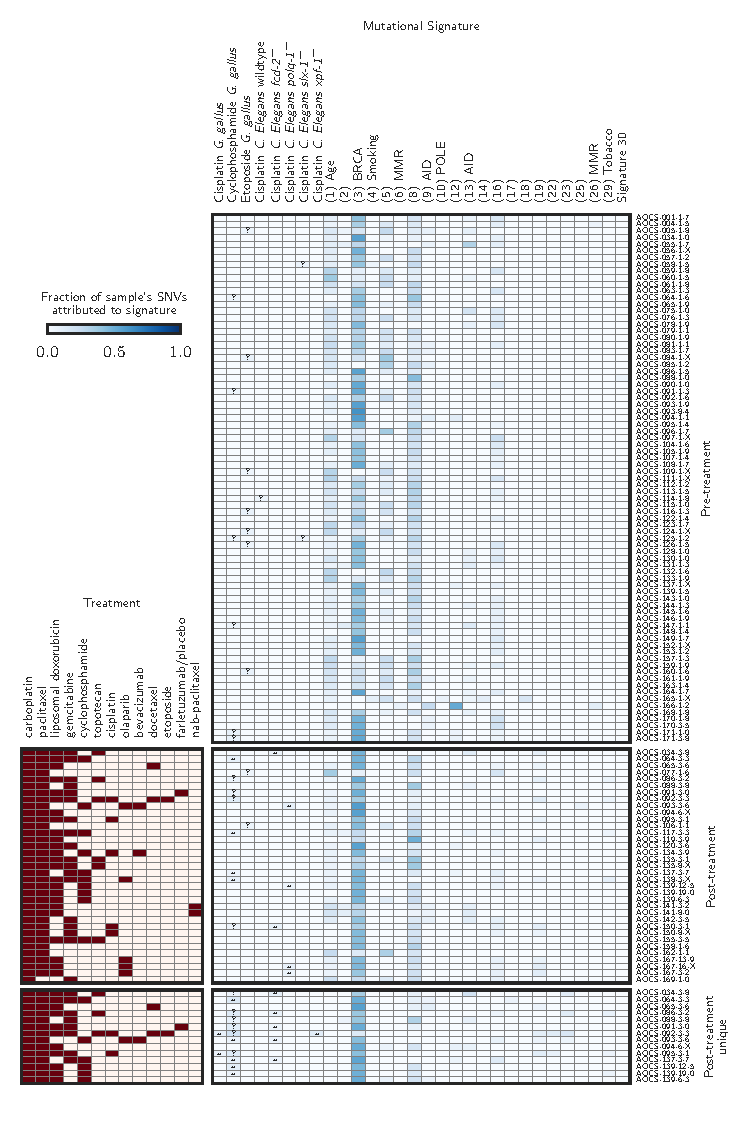
\includegraphics[scale=1.0]{figures/supplementary_signatures.pdf}
\caption{\textbf{Mutational signature deconvolutions for all samples.} The symbols are as in main text figure~\ref{fig:signatures}.}
\label{fig:supp_signatures}
\end{figure}

\begin{figure}
\centering
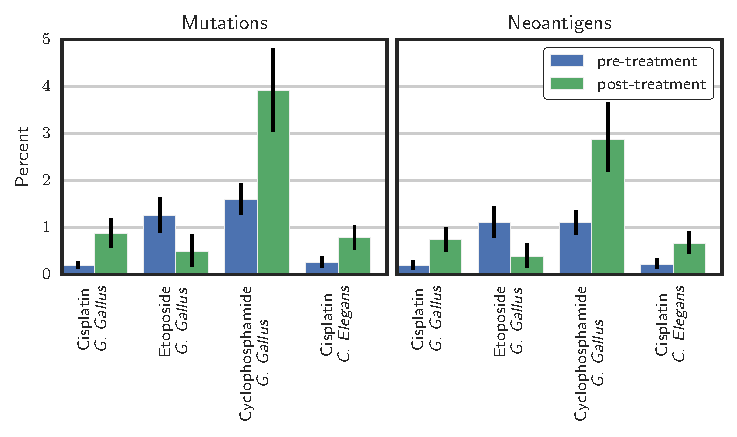
\includegraphics[scale=1.0]{figures/sources_of_mutations_and_neoantigens_ungrouped.pdf}
\caption{\textbf{Contributions of chemotherapy-associated mutational signatures to mutations and neoantigens, as a fraction of total.}}
\label{fig:supp_sources}
\end{figure}

\begin{figure}
\centering
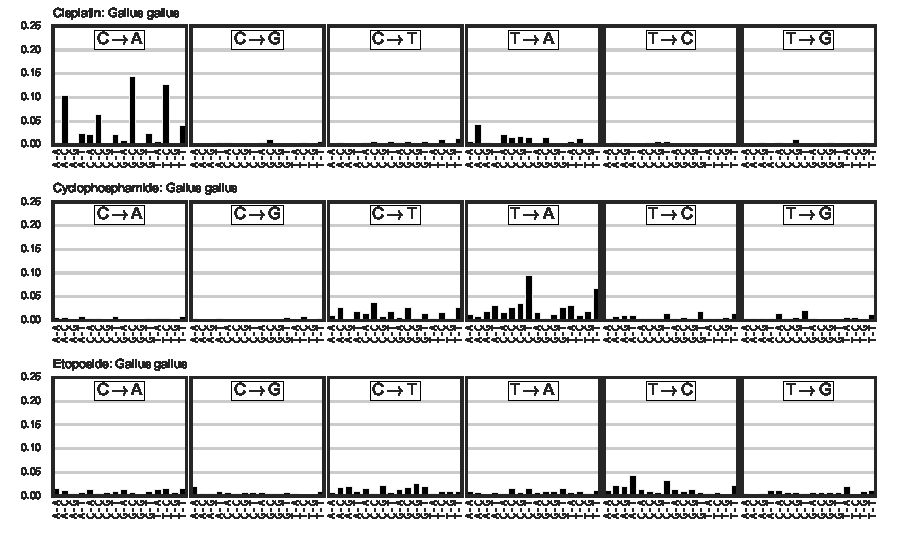
\includegraphics[scale=1.0]{figures/extracted_signatures_chicken.pdf}
\caption{Mutational signatures extracted from \cite{Szikriszt_2016}}
\label{fig:supp_extracted_signatures_chicken}
\end{figure}

\begin{figure}
\centering
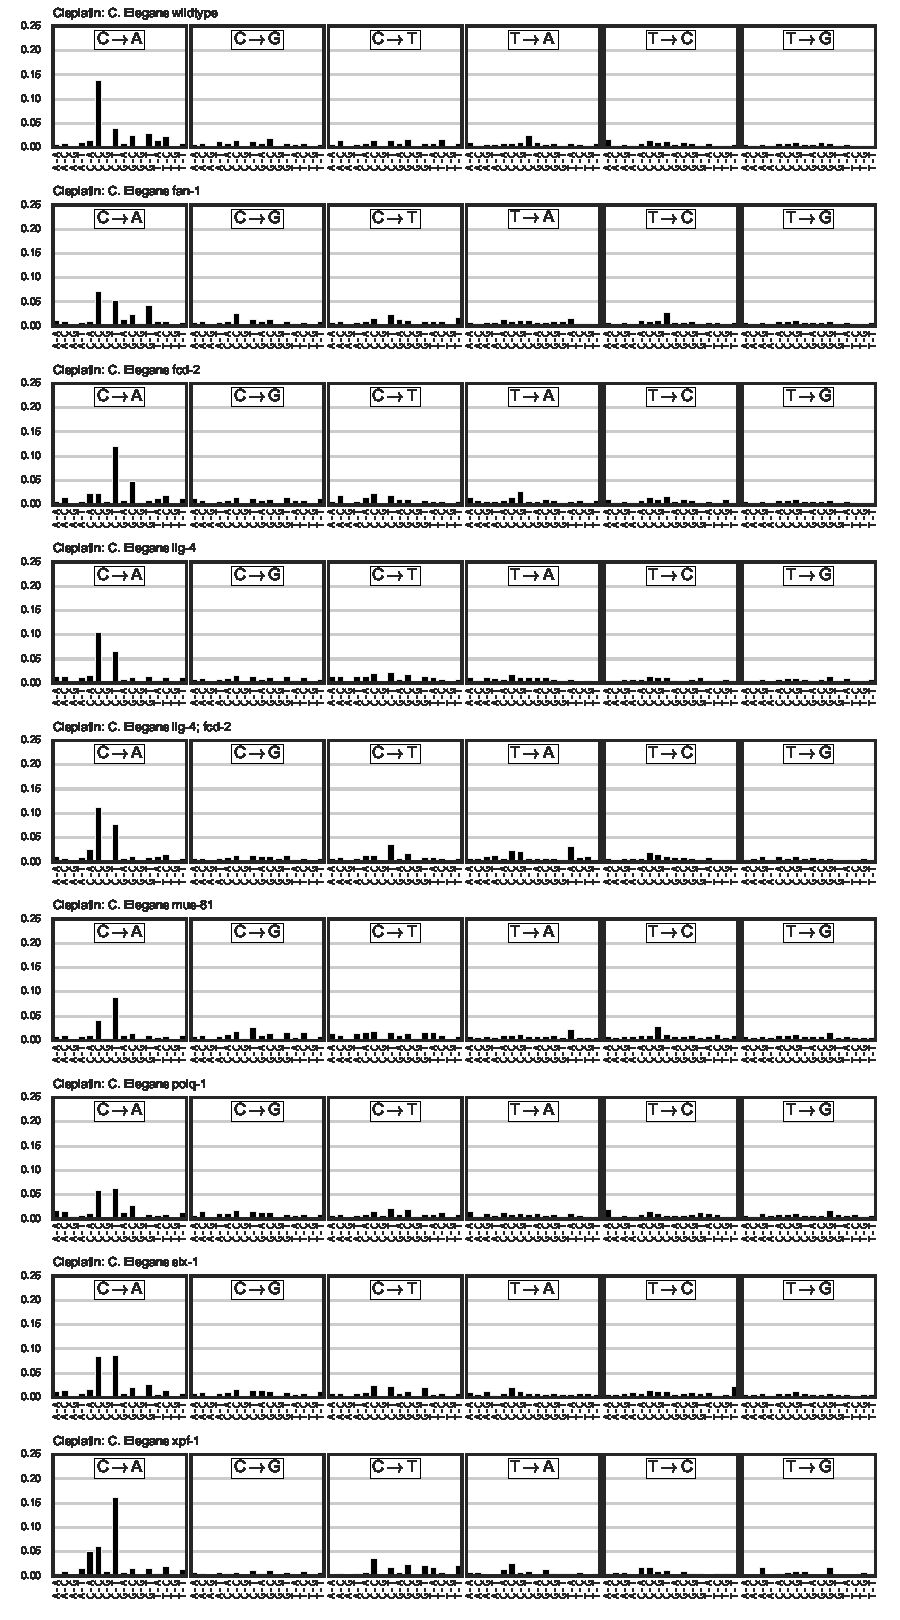
\includegraphics[scale=1.0]{figures/extracted_signatures_worm.pdf}
\caption{Mutational signatures extracted from \cite{Meier_2014}}
\label{fig:supp_extracted_signatures_worm}
\end{figure}

\FloatBarrier
